\section{Implementation description}
\label{sec:description}

\subsection{\texttt{optimize()}}
\begin{figure}[h!]
\centering
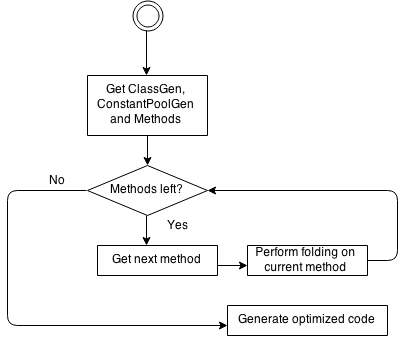
\includegraphics[scale=0.6]{figures/overview}
\caption{The control flow for \texttt{optimize}}
\label{fig:overview}
\end{figure}
\textbf{Brief: }Calls \texttt{performFolding} for every method.\\

First it a new \texttt{ClassGen} object is created from which the \texttt{ConstantPool} and the unoptimized methods are retrieved. Then,  a loop iterates over these methods and calls \texttt{performFolding} for each one,  passing the current method, the \texttt{ConstantPoolGen} and the \texttt{ClassGen} object. Once there are no more methods remaining, the optimized code is generated.

\subsection{\texttt{performFolding(ClassGen gen, ConstantPoolGen cpgen, Method method)}}
\label{subsec:performfolding}
\textbf{Brief: }Performs simple, constant and dynamic folding on method \texttt{m}, invoking itself recursively until no further optimization is possible. \\

\subsubsection{Data Structures}
It uses five major data structures to always keep track of the algorithm's and method code's state:

\begin{itemize}
\item \textbf{\texttt{constantStack}}: Simulates the constant stack and contains only the most recent values.
\item \textbf{\texttt{instructionStack}}: Contains the actual processed instructions and all those that will be removed at the end.
\item \textbf{\texttt{pushInstrIndexStack}}: Contains indices of all push instructions of the current optimisation step in the order they appeared in the bytecode.
\item \textbf{\texttt{instructionMap}}: Instead of completely removing the store operation, it is saved in this data structure in case it is need at a later point in the code.
\item \textbf{\texttt{constantMap}}: When a store instruction is read, the topmost constant is popped from the \texttt{\texttt{constantStack}} and stored in a local variable table. This \texttt{constantMap} simulates that table, so that we always have access to the most recent value of a variable.
\end{itemize}

\subsubsection{Other Variables and Data Structures}
\begin{itemize}
\item \textbf{\texttt{methodCode}}: Code of the method, containing a header and the \texttt{instList}.
\item \textbf{\texttt{instList}}: List consisting of references to all instructions (\texttt{InstructionHandles}) in the method's code
\item \textbf{\texttt{remove}}: Flag that indicates if an instruction can be removed, i.e. an interaction with the \texttt{instructionStack} is necessary.
\item \textbf{\texttt{changed}}: Flag that indicates whether the instructions have been optimized (i.e. the original code has changed) 
\item \textbf{\texttt{instrPointer}}: Indicates the number of instructions on the \texttt{instructionStack}. Incremented only when an instruction is added and decremented when instructions are popped from the stack.
\end{itemize}

\subsubsection{Code Description}
The \texttt{performFolding} method does all three types of folding: simple, constant, and dynamic. It first retrieves the method's code from the method object and then receives all instructions as a list (\texttt{instList}). Then it iterates over the instruction list using the instruction \texttt{handle} (pointer to specific instruction in \texttt{instList}). Each handle is checked to see if it is a valid instruction - if it is not, then the instruction is ignored and the next handle is addressed. The algorithm determines an instruction’s type by making use of Java's \texttt{instanceof} operator.

When the loop is finished or has been interrupted by an optimization, the \texttt{changed} flag is checked. If \texttt{changed} is \texttt{true}, the actual reduction step is performed (\texttt{performReduction}, subsection \ref{subsec:performreduction}), followed by a clean up (\texttt{cleanUpInstructionList}, subsection \ref{subsec:cleanup}) of the \texttt{instList}. The latter is necessary to get rid of store-related instructions that do not have an appropriate load and are therefore useless. After the clean up, a new method is created which replaces the current one, and \texttt{performFolding} is invoked with this new method (i.e. the optimized code of the original method) as actual parameter.

As explained before, it checks whether each instruction is of type Push (direct/indirect), Conversion, Store, Arithmetic Operation or Comparison (see section \ref{sec:classification} for further explanation).

\paragraph{Push instructions.}
\begin{figure}[h!]
\centering
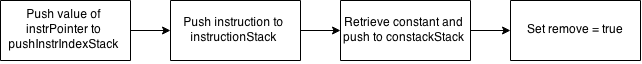
\includegraphics[scale=0.7]{figures/push}
\caption{Control flow for push instructions}
\end{figure}
First, the instruction is pushed to the \texttt{instructionStack}, and the loaded constant is pushed to the \texttt{constantStack}. The flag \texttt{remove} is also set to \texttt{true} which indicates that all following instructions must be taken into account.     
In the next iteration, if \texttt{remove} is set to \texttt{true}, it checks the next instruction. If the instruction is not of type Push, it executes specific code according to the instruction type.

It is worth mentioning, that we distinguish between \textit{direct} and \textit{indirect} push operations. Direct push instructions immediately push constants to the stack. Indirect push instructions first load the constant from the local variable table and then push it tpo the constant stack. The only indirect push instructions are those of type \texttt{load}.

\paragraph{Store instruction.}
\begin{figure}[h!]
\centering
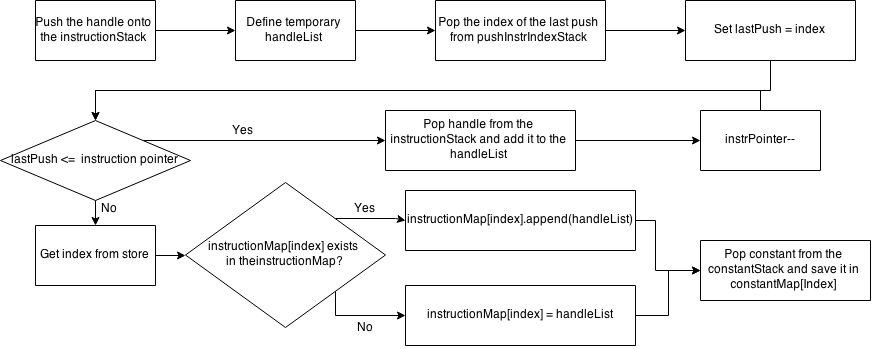
\includegraphics[scale=0.5]{figures/store}
\caption{Control flow for store instructions}
\end{figure}

Firstly, the instruction’s \texttt{handle} is added to the \texttt{instructionStack} and a temporary handle list (\texttt{instructionHandles}) is defined. Then, a variable called \texttt{lastPush} is created and initialized with the index of the last push operation, i.e. the topmost element of the \texttt{pushInstrIndexStack}. Then a while loop iterates over the \texttt{instructionStack} and in each iterations pops the topmost instruction and adds it to \texttt{instructionHandles}. Finally, \texttt{instrPointer} is decreased. This repeats until all handles that have been added since the last push operation are popped from the \texttt{instructionStack}. 
In this way, the algorithm can even consider conversion instructions which are placed between the last push and the current store instruction. Hence, it pops all handles that are necessary for this store instruction \footnote{This might not even be necessary. However, due to lack of time, we kept it in our implementation, because it works fine.}. Once the loop has ended, it stores the value in the \texttt{constantMap}, where the key is the \texttt{store} instruction’s reference index. It also saves the \texttt{handleList} in the \texttt{instructionMap}, again using the reference index as key. In case of dynamic folding, the \texttt{handleList} is added to the existing one in \texttt{instructionMap}. In case anything goes wrong, the containers will be cleared and remove is set to false, meaning that the pattern matching process will start from new in the next iteration.

\paragraph{Conversion instructions.}
\begin{figure}[h!]
\centering
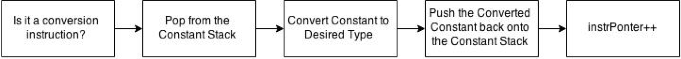
\includegraphics[scale=0.6]{figures/conversion}
\caption{Control flow for conversion instructions}
\end{figure}

The topmost constant on the \texttt{constantStack} is popped and converted to the desired type. It is then pushed back to the \texttt{constantStack} and the particular instruction handle is pushed to the \texttt{instructionStack}. Finally, the \texttt{instrPointer} is incremented. 

\paragraph{Arithmetic instructions.}
\begin{figure}[h!]
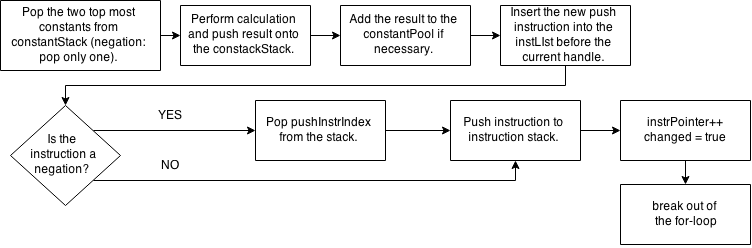
\includegraphics[scale=0.6]{figures/arithmetic}
\caption{Control flow for arithmetic operations}
\end{figure}

If it is an arithmetic instruction, the two topmost constants are popped from the \texttt{constantStack}. In case of a negation, only the one topmost constant is popped. The desired calculation is then performed and the result is pushed to the \texttt{constantStack} and, is necessary, added to the general constant pool. Next, a new push instruction is inserted within the instruction list directly before the current handle. The type of this instruction depends on the size of the variable. In that way, the algorithm does not add constants to the constant pool when they can be also pushed directly (using \texttt{sipush, bipush, i/l/d/fconst}).\\
If the instruction is not a negation, the topmost push instruction index is popped from \texttt{pushInstrIndexStack}. This is because two push operations are involved in the arithmetic operation and therefore the removal should not stop when reaching the last, but when reaching the second last push instruction on the \texttt{pushInstrIndexStack}. After that, the instruction is pushed to the \texttt{instructionStack} and the \texttt{instrPointer} is incremented by one. Also, the \texttt{changed} flag is set to \texttt{true}. Finally, the function breaks out of the loop, since the algorithm only performs one optimization at a time.

\paragraph{Comparison instructions.}
\begin{figure}[h!]
\centering
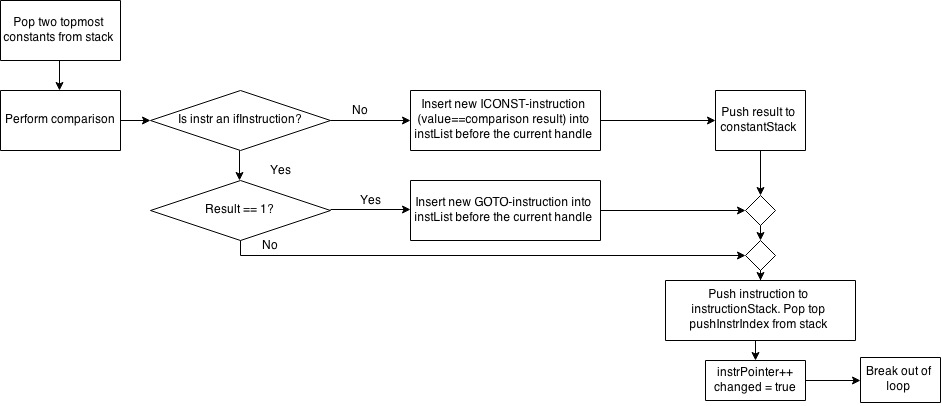
\includegraphics[scale=0.45]{figures/comparison}
\caption{Control flow for comparison operations}
\end{figure}

If the instruction’s type is a comparison, the topmost constants are popped from the stack before the comparison is performed. Since particularly if-instructions imply a jump if the comparison evaluates to \texttt{true}, in that particular case the algorithm checks if the result is equal to 1, i.e. \texttt{true}. If this is the case, a new \texttt{goto} instruction is inserted into the \texttt{instList} before the current handle and the instruction is pushed to the \texttt{instructionStack}. This means nothing more than: the current instruction is replaced by a \texttt{goto} instruction. If the result is equal to 0, no new instruction is added and the current one will simply be removed.\\
If the instruction is not an if-instruction, the current \texttt{handle} is replaced by an \texttt{iconst} instruction. Afterwards, the \texttt{instrPointer} is incremented and the \texttt{changed} flag is set to \texttt{true}. Finally, the function breaks out of the loop, since the algorithm only performs one optimization at a time.

\subsection{\texttt{performReduction(\\
\hspace{2cm}Deque<InstructionHandle> instructionStack, \\
\hspace{2cm}InstructionList instList, \\
\hspace{2cm}Deque<Integer> pushInstrIndexStack, \\
\hspace{2cm}int instrPointer)}}
\label{subsec:performreduction}
\textbf{Brief: }Removes all instructions that are not needed any more once the optimization was successful. \\

This method deletes all instructions in the \texttt{instList} that are on the \texttt{instructionStack} between the last push and the top. If one of the deleted handles is still targeted by branch instructions, their targets are set to the parameter \texttt{newHandle} and the \texttt{TargetLostException} therefore handled accordingly.
%\clearpage
\subsection{\texttt{cleanUpInstructionList(\\
\hspace{2cm}Map<Integer,ArrayList<InstructionHandle> > map,\\
\hspace{2cm}InstructionList instList,\\
\hspace{2cm}InstructionHandle newHandle)}}
\label{subsec:cleanup}
\textbf{Brief: }Removes all instructions that are not needed any more once the optimization was successful. \\

This deletes all unneeded instructions from the instruction list. This is necessary to get rid of store related instructions that do not have an appropriate load and are therefore not needed any more. \\
First, a list is defined which will store all the entries that will be removed (\texttt{removeEntries}). Then the algorithm iterates over all entries in the \texttt{instructionMap} and checks whether the current \texttt{instList} contains a load with the same reference as the current \texttt{entry}’s key. If not, the \texttt{entry} is stored in \texttt{removeEntries} for later removal.\\
If one of the deleted handles is still targeted by branch instructions, their targets are set to the parameter \texttt{newHandle} and the \texttt{TargetLostException} therefore handled accordingly.